\input templates/header
\title[ASD - Divide-et-impera]{\textbf{Algoritmi e Strutture Dati}\\[24pt]Divide-et-impera}

\usepackage{tikz}
\usepackage{xmpmulti}
\usepackage{listings}

\lstset{
  basicstyle=\ttfamily,
  columns=fullflexible,
  keywordstyle=\color{red}\bfseries,
  commentstyle=\color{blue},
  showstringspaces=false,
}

\graphicspath{{figs/12/}}

\begin{document}

%-------------------------------------------------------------------------
\FrameTitle{}

%-------------------------------------------------------------------------
\FrameContent


%%%%%%%%%%%%%%%%%%%%%%%%%%%%%%%%%%%%%%%%%%%%%%%%%%%%%%%%%%%%%%%%%%%%%%%%%%
\section{Introduzione}



%-------------------------------------------------------------------------
\begin{frame}{Risoluzione problemi}

\vspace{-9pt}
\BB{Dato un problema}
\BIL
\item Non ci sono "ricette generali" per risolverlo in modo efficiente
\item Tuttavia, è possibile evidenziare quattro fasi
\BI
\item \alert{Classificazione del problema}
\item \alert{Caratterizzazione della soluzione}
\item \alert{Tecnica di progetto}
\item \alert{Utilizzo di strutture dati}
\EI
\item Queste fasi non sono necessariamente sequenziali
\EIL

\end{frame}


%-------------------------------------------------------------------------
\begin{frame}{Classificazione dei problemi}

\vspace{-9pt}
\begin{myboxtitle}[Problemi decisionali]
\BIL
\item Il dato di ingresso soddisfa una certa proprietà?
\item Soluzione: risposta sì/no
\item Esempio: Stabilire se un grafo è connesso
\EIL
\end{myboxtitle}
\begin{myboxtitle}[Problemi di ricerca]
\BIL
\item Spazio di ricerca: insieme di "soluzioni" possibili
\item Soluzione ammissibile: soluzione che rispetta certi vincoli
\item Esempio: posizione di una sottostringa in una stringa
\EIL
\end{myboxtitle}

\end{frame}

%-------------------------------------------------------------------------
\begin{frame}{Classificazione dei problemi}

\vspace{-9pt}
\begin{myboxtitle}[Problemi di ottimizzazione]
\BIL
\item Ogni soluzione è associata ad una funzione di costo
\item Vogliamo trovare la soluzione di costo minimo
\item Esempio: cammino più breve fra due nodi
\EIL
\end{myboxtitle}

\end{frame}

%-------------------------------------------------------------------------
\begin{frame}{Definizione matematica del problema}

\vspace{-9pt}
\BB{\EE fondamentale definire bene il problema in modo formale}
	\BIL
	\item Spesso la formulazione è banale...
	\item ... ma può suggerire una prima idea di soluzione
	\item Esempio: Data una sequenza di $n$ elementi, una permutazione ordinata 
	è data dal minimo seguito da una permutazione ordinata dei restanti $n-1$ elementi
	(Selection Sort)
	\EIL
	
\medskip
\BB{La definizione matematica può suggerire una  possibile tecnica}
	\BIL
	\item \alert{Sottostruttura ottima} $\rightarrow$ \alert{Programmazione dinamica}
	\item \alert{Proprietà greedy} $\rightarrow$ \alert{Tecnica greedy}
	\EIL
    
\end{frame}


%-------------------------------------------------------------------------
\begin{frame}{Tecniche di soluzione problemi}

\vspace{-9pt}
\begin{myboxtitle}[Divide-et-impera]
\BI
\item Un problema viene suddiviso in sotto-problemi indipendenti, che vengono
risolti ricorsivamente (top-down)
\item Ambito: problemi di decisione, ricerca
\EI
\end{myboxtitle}

\begin{myboxtitle}[Programmazione dinamica]
\BI
\item La soluzione viene costruita (bottom-up) a partire da un insieme di
sotto-problemi potenzialmente ripetuti
\item Ambito: problemi di ottimizzazione
\EI
\end{myboxtitle}
\begin{myboxtitle}[Memoization (o annotazione)]
\BI
\item Versione top-down della programmazione dinamica
\EI
\end{myboxtitle}


\end{frame}

%-------------------------------------------------------------------------
\begin{frame}{Tecniche di soluzione problemi}

\vspace{-9pt}
\begin{myboxtitle}[Tecnica greedy]
\BI
\item Approccio "ingordo": si fa sempre la scelta localmente ottima
\EI
\end{myboxtitle}

\begin{myboxtitle}[Backtrack]
\BI
\item Procediamo per "tentativi", tornando ogni tanto sui nostri passi
\EI
\end{myboxtitle}

\begin{myboxtitle}[Ricerca locale]
\BI
\item La soluzione ottima viene trovata "migliorando" via via soluzioni esistenti
\EI
\end{myboxtitle}

\begin{myboxtitle}[Algoritmi probabilistici]
\BI
\item Meglio scegliere con giudizio (ma in maniera costosa) o scegliere a caso ("gratuitamente")
\EI
\end{myboxtitle}

\end{frame}

\begin{frame}{Divide-et-impera}
    
\vspace{-9pt}
\BB{Tre fasi}
\BIL
\item \alert{Divide}: Dividi il problema in sotto-problemi più piccoli e indipendenti
\item \alert{Impera}: Risolvi i sotto-problemi ricorsivamente
\item \alert{Combina}: "unisci" le soluzioni dei sottoproblemi
\EIL

\medskip
\BB{Non esiste una ricetta "unica" per divide-et-impera}
\BIL
\item Merge Sort: "divide" banale, "combina" complesso
\item Quicksort: "divide" complesso, niente fase di "combina"
\item \EE necessario uno sforzo creativo
\EIL

\end{frame}

\begin{frame}{Minimo divide-et-impera}
	
\vspace{-9pt}
\begin{Procedure}
\caption[A]{\INTEGER\ \textsf{minrec}($\INTEGER[\,]\ A$, \INTEGER $i$, \INTEGER $j$)}
\eIf{$i \Eq j$}{
  \Return $A[i]$\;
}{
	$m = \lfloor (i+j)/2 \rfloor$\;
	\Return $\textsf{min}(\textsf{minrec}(A,i,m), \textsf{minrec}(A,m+1,j))$\;
}
\end{Procedure}

\vspace{-12pt}
\begin{myboxtitle}[Complessità]
\begin{overprint}
\onslide<1|handout:0>
~
\onslide<2|handout:0>
\[
  T(n) = \begin{cases} 
		2T(n/2) + 1 & n>1 \\
		1 & n=1
	\end{cases}
\]
\onslide<3|handout:1>
\[
  T(n) = \begin{cases} 
		2T(n/2) + 1 & n>1 \\
		1 & n=1
	\end{cases}
\]
$T(n) = \Theta(n)$ -- Non ne vale la pena!
\end{overprint}
\end{myboxtitle}

\end{frame}


\section{Torri di Hanoi}

%-------------------------------------------------------------------------
\begin{frame}{Le torri di Hanoi}
	
\vspace{-12pt}
\TwoColsCustom{0.6}{0.37}{
\BB{Gioco matematico}
\BI
\item tre pioli
\item $n$ dischi di dimensioni diverse
\item Inizialmente, i dischi sono impilati in ordine decrescente 
nel piolo di sinistra
\EI
}{
\IG{1.0}{hanoi.jpg}
\vspace{-10pt}
{\tiny \url{https://it.wikipedia.org/wiki/File:Tower_of_Hanoi.jpeg}}
}


\BB{Scopo del gioco}
\BI
\item Impilare in ordine decrescente i dischi sul piolo di destra
\item Senza mai impilare un disco più grande su uno più piccolo
\item Muovendo al massimo un disco alla volta
\item Utilizzando il piolo centrale come appoggio
\EI

\end{frame}



%-------------------------------------------------------------------------
\begin{frame}{Le torri di Hanoi}
\vspace{-12pt}
\begin{Procedure}
\caption[A]{\textsf{hanoi}(\INTEGER\ $n$, \INTEGER\ $\mathit{src}$, \INTEGER\ $\mathit{dest}$, \INTEGER\ $\mathit{middle}$)}

\eIf{$n \Eq 1$}
{
  \PRINT $\mathit{src} \rightarrow \mathit{dest}$\;
}
{
  $\textsf{hanoi}(n-1, \mathit{src}, \mathit{middle}, \mathit{dest})$\;
  \PRINT $\mathit{src} \rightarrow \mathit{dest}$\;
 	$\textsf{hanoi}(n-1, \mathit{middle}, \mathit{dest}, \mathit{src})$\;
}
\end{Procedure}

\TwoCols{
\vspace{-6pt}
\BB{\textbf{Divide-et-impera}}
\BIL
\item $n-1$ dischi da $\mathit{src}$ a $\mathit{middle}$
\item $1$ disco da $\mathit{src}$ a $\mathit{dest}$
\item $n-1$ dischi da $\mathit{middle}$ a $\mathit{dest}$
\EI
}{
\begin{overprint}
\onslide<0|handout:1>

\includegraphics[width=\textwidth]{hanoi-0.png}
\onslide<1-39|handout:0>
\multiinclude[<+>][format=png,start=0,end=38,graphics={width=\textwidth}]{hanoi}
{\tiny \url{https://it.wikipedia.org/wiki/Torre_di_Hanoi\#/media/File:Tower_of_Hanoi_4.gif}}
\end{overprint}
}
\end{frame}

\begin{frame}{Le torri di Hanoi}
\vspace{-12pt}
\begin{Procedure}
\caption[A]{\textsf{hanoi}(\INTEGER\ $n$, \INTEGER\ $\mathit{src}$, \INTEGER\ $\mathit{dest}$, \INTEGER\ $\mathit{middle}$)}

\eIf{$n=1$}
{
  \PRINT $\mathit{src} \rightarrow \mathit{dest}$\;
}
{
  $\textsf{hanoi}(n-1, \mathit{src}, \mathit{middle}, \mathit{dest})$\;
  \PRINT $\mathit{src} \rightarrow \mathit{dest}$\;
 	$\textsf{hanoi}(n-1, \mathit{middle}, \mathit{dest}, \mathit{src})$\;
}
\end{Procedure}

\vspace{-6pt}
\begin{myboxtitle}[Costo computazionale]
\begin{overprint}
\onslide<1|handout:0>
?
\onslide<2|handout:1>
\BIL
\item Ricorrenza: $T(n) = 2T(n-1)+1$
\item Costo computazionale? \alert{$O(2^n)$}
\item Questa soluzione è ottima (si può dimostrare)
\EIL
\end{overprint}
\end{myboxtitle}
\end{frame}


\section{Quicksort}

\begin{frame}{Quicksort (Hoare, 1961)}
	
\vspace{-9pt}
\begin{myboxtitle}[Algoritmo di ordinamento basato su divide-et-impera]
\BI
\item Caso medio: $O(n \log n)$
\item Caso pessimo: $O(n^2)$
\EI
\end{myboxtitle}

\begin{myboxtitle}[Caso medio vs caso pessimo]
\BI
\item Il fattore costante di Quicksort è migliore di Merge Sort
\item "In-memory": non utilizza memoria addizionale
\item Tecniche "euristiche" per evitare il caso pessimo
\item Quindi spesso è preferito ad altri algoritmi
\EI
\end{myboxtitle}

\BB{
\footnotesize
R. Sedgewick, "\alert{\emph{Implementing Quicksort Programs}}". Communications of the ACM, 21(10):847-857, 1978.
\url{http://portal.acm.org/citation.cfm?id=359631}
}
\end{frame}


\begin{frame}{Quicksort}

\vspace{-9pt}
\begin{myboxtitle}[Input]
\BI
\item Vettore $A[1 \ldots n]$, 
\item Indici $\Primo$, $\Ultimo$ tali che $1 \leq \Primo \leq \Ultimo \leq n$
\EI
\end{myboxtitle}

\begin{myboxtitle}[Divide]
\BIL
\item Sceglie un valore $p \in A[\Primo \ldots \Ultimo]$ 
  detto \alert{perno} (\alert{pivot})
\item Sposta gli elementi del vettore $A[\Primo \ldots \Ultimo]$ in modo che:

\IG{0.7}{quicksort-spiegazione.pdf}


% $\displaystyle
% \begin{aligned}
%   \forall i \in [\Primo \ldots j - 1]: &A[i] \leq p \\
%   \forall i \in [j + 1 \ldots \Ultimo]: &A[i] \geq p \\
%  \end{aligned}
%   $
\item L'indice $j$ del perno va calcolato opportunamente
\EIL
\end{myboxtitle}

\end{frame}

\begin{frame}{Quicksort}

\vspace{-9pt}
\begin{myboxtitle}[Impera]
Ordina i due sottovettori $A[\Primo \ldots j  -  1]$ e $A[j + 1 \ldots \Ultimo]$\\ 
richiamando ricorsivamente Quicksort
\end{myboxtitle}

\begin{myboxtitle}[Combina]
Non fa nulla: infatti,
\BI
\item il primo sottovettore,
\item $A[j]$,
\item il secondo sottovettore 
\EI
formano già un vettore ordinato
\end{myboxtitle}

\end{frame}


\begin{frame}{Quicksort -- \textsf{pivot}()}

\small
\vspace{-9pt}
\TwoColsCustom{0.58}{0.42}{
\begin{Procedure}
\caption[A]{\INTEGER \Perno($\Item[\,]\ A$, \INTEGER $\Primo$, \INTEGER $\Ultimo$)}
$\Item\ \mathit{pivot} = A[\Primo]$\;
$\INTEGER\ j = \Primo$\;
\For{$i = \Primo+1$ \TO\ $\Ultimo$}
{
  \If{$A[i] <\mathit{ pivot}$}
  {
    $j = j + 1$\;
	$\Swap(A,i,j)$\;
  }
}
$A[\Primo] = A[j]$\;
$A[j] = \mathit{pivot}$\;
\Return{$j$}
\end{Procedure}
}
{
\begin{Procedure}
\caption[A]{\Swap($\Item[\,]\ A$, \INTEGER $i$, \INTEGER $j$)}
$\Item\ \mathit{temp} = A[i]$\;
$A[i] = A[j]$\;
$A[j] = \mathit{temp}$\;
\end{Procedure}
}

\end{frame}


%-------------------------------------------------------------------------
\begin{frame}{Funzionamento \textsf{pivot}()}

\vspace{-9pt}
\begin{overprint}
\includegraphics<1|handout:1>[width=0.95\textwidth]{pivot1}
\includegraphics<2|handout:2>[width=0.95\textwidth]{pivot2}
\end{overprint}

\end{frame}

\begin{frame}{Quicksort -- Procedura principale}
    
\vspace{-9pt}
\begin{Procedure}
\caption[A]{\Quicksort($\Item[\,]\ A$, \INTEGER $\Primo$, \INTEGER $\Ultimo$)}
\If{$\Primo < \Ultimo$}
{
  $\INTEGER\ j = \Perno(A, \Primo, \Ultimo)$\;
  $\Quicksort(A, \Primo, j  -  1)$\;
  $\Quicksort(A, j + 1, \Ultimo)$\;
}
\end{Procedure}
\end{frame}


%-------------------------------------------------------------------------
\begin{frame}{Svolgimento ricorsione}

\vspace{-12pt}
\begin{center}
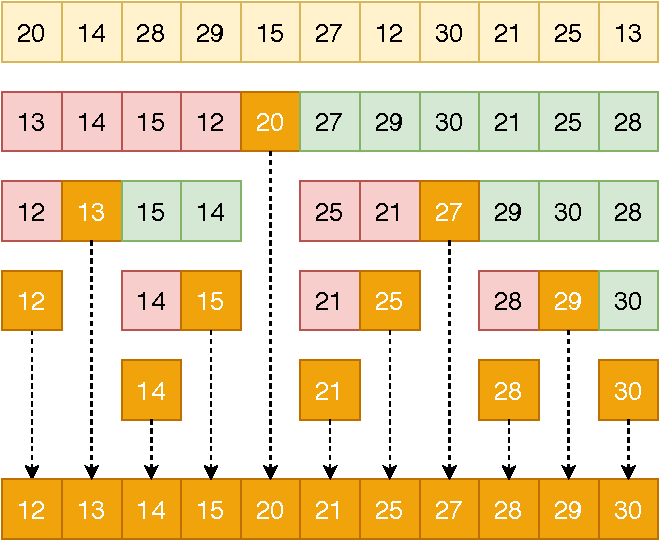
\includegraphics[width=0.75\textwidth]{quicksort-esecuzione}
\end{center}

\end{frame}

%-------------------------------------------------------------------------
\begin{frame}{Quicksort: Complessità computazionale}

\vspace{-9pt}
\BB{Costo di $\Perno()$?}
\pause
\BI
\item $\Theta(n)$
\EI

\BB{Costo Quicksort: caso pessimo?}
\pause
\BI
\item Il vettore di dimensione $n$ viene diviso in due sottovettori di 
dimensione $0$ e $n-1$
\item $T(n) = T(n-1)+T(0)+\Theta(n) = T(n-1) + \Theta(n) = \Theta(n^2)$
\EI

\BB{Costo Quicksort: caso ottimo?}
\pause
\BI
\item Dato un vettore di dimensione $n$, viene sempre diviso in due 
sottoproblemi di dimensione $n/2$
\item $T(n) = 2T(n/2)+\Theta(n) = \Theta(n \log n)$
\EI

\end{frame}

%-------------------------------------------------------------------------
\begin{frame}{Quicksort: Complessità computazionale}

\vspace{-9pt}
\BB{Partizionamenti parzialmente bilanciati}
\BIL
\item Il partizionamento nel caso medio di Quicksort è molto più vicino al caso ottimo che al caso peggiore
\item Esempio: Partizionamento 9-a-1:	

\vspace{-6pt}
\[T(n) = T(n/10)+T(9n/10)+cn = \Theta(n \log n)\]
\item Esempio: Partizionamento 99-a-1:	

\vspace{-6pt}
\[T(n) = T(n/100)+T(99n/100)+cn  = \Theta(n \log n)\]
\EIL
\BB{Note}
\BIL
\item In questi esempi, il partizionamento ha proporzionalità limitata
\item I fattori moltiplicativi possono essere importanti
\EIL
\end{frame}


%-------------------------------------------------------------------------
\begin{frame}{Quicksort: Complessità computazionale}

\vspace{-9pt}
\BB{Caso medio}
\BIL
\item Il costo dipende dall'ordine degli elementi, non dai loro valori
\item Dobbiamo considerare tutte le possibili permutazioni
\item Difficile dal punto di vista analitico
\EIL

\BB{Caso medio: un'intuizione}
\BIL
\item Alcuni partizionamenti saranno parzialmente bilanciati
\item Altri saranno pessimi
\item In media, questi si alterneranno nella sequenza di partizionamenti
\item I partizionamenti parzialmente bilanciati “dominano” quelli pessimi
\EIL
\end{frame}

%-------------------------------------------------------------------------
\begin{frame}{Quicksort: Selezione pivot euristica}

\BB{Tecnica euristica: selezionare il valore mediano fra il primo elemento, l'ultimo elemento e il valore nella posizione centrale}

\begin{Procedure}
\caption[A]{\INTEGER \Perno($\Item[\,]\ A$, \INTEGER $\Primo$, \INTEGER $\Ultimo$)}
$\INTEGER\ m = \lfloor (\Primo+\Ultimo)/2 \rfloor$\;
\If(\REMF{Sposta il massimo in ultima posizione}){$A[\Primo] > A[\Ultimo]$}{
  $\Swap(A,\Primo,\Ultimo)$\;
}
\If(\REMF{Sposta il massimo in ultima posizione}){$A[m] > A[\Ultimo]$}{
  $\Swap(A,m,\Ultimo)$\;
}
\If(\REMF{Sposta il mediano in prima posizione}){$A[m] > A[\Primo]$}{
  $\Swap(A,m,\Primo)$\;
}
$\Item\ \mathit{pivot} = A[\Primo]$\;
[...]\;
\end{Procedure}

\end{frame}

\begin{frame}<handout:0>[fragile,shrink=20]{\url{https://xkcd.com/1185/}}
\vspace{-12pt}
\begin{lstlisting}
define JobInterviewQuicksort(list):
  Ok so you choose a pivot
  Then divide the list in half
  for each half:
    check to see if it's sorted
      no, wait, it doesn't matter
    compare each element to the pivot
      the bigger ones go in a new list
      the equal ones go into, uh
      the second list from before
    hang on, let me name the lists
      this is list A
      the new one is list B
    put the big ones into list B
    now take the second list
      call it list, uh, A2
    which one was the pivot in?
    scratch all that
    it just recursively calls itself
    until both lists are empty
      right?
    not empty, but you know what I mean
  am I allowed to use the standard libraries?
\end{lstlisting}

\end{frame}



\section{Algoritmo di Strassen}

\begin{frame}{Moltiplicazione matrici}

\vspace{-9pt}
\TwoColsCustom{0.28}{0.70}{
\begin{align*}
C &= A \times B\\
c_{i,j} &= \alert{\sum_{k=1}^{n_k} a_{i,k} \cdot b_{k,j}}\\
T(n) &= \Theta(n_i \cdot n_k \cdot n_j) \\
							 &= \Theta(n^3)
\end{align*}
}{
\vspace{-12pt}
\begin{Procedure}
\caption[A]{\textsf{matrixProduct}($\REAL[\,][\,]\ A, B, C,\ \INTEGER\ n_i, n_k, n_j$)}	

\For(\Comment*[f]{Righe}){$i = 1$ \TO\ $n_i$}
{
  \For(\Comment*[f]{Colonne}){$j = 1$ \TO\ $n_j$}
  {
\alert{
     $C[i,j] = 0$\;
     \For{$k = 1$ \TO\ $n_k$}
     {
        $C[i,j] = C[i,j] + A[i,k] \cdot B[k,j]$\;
     }
}
  }
}
\end{Procedure}
}
\vspace{-12pt}
\begin{center}
	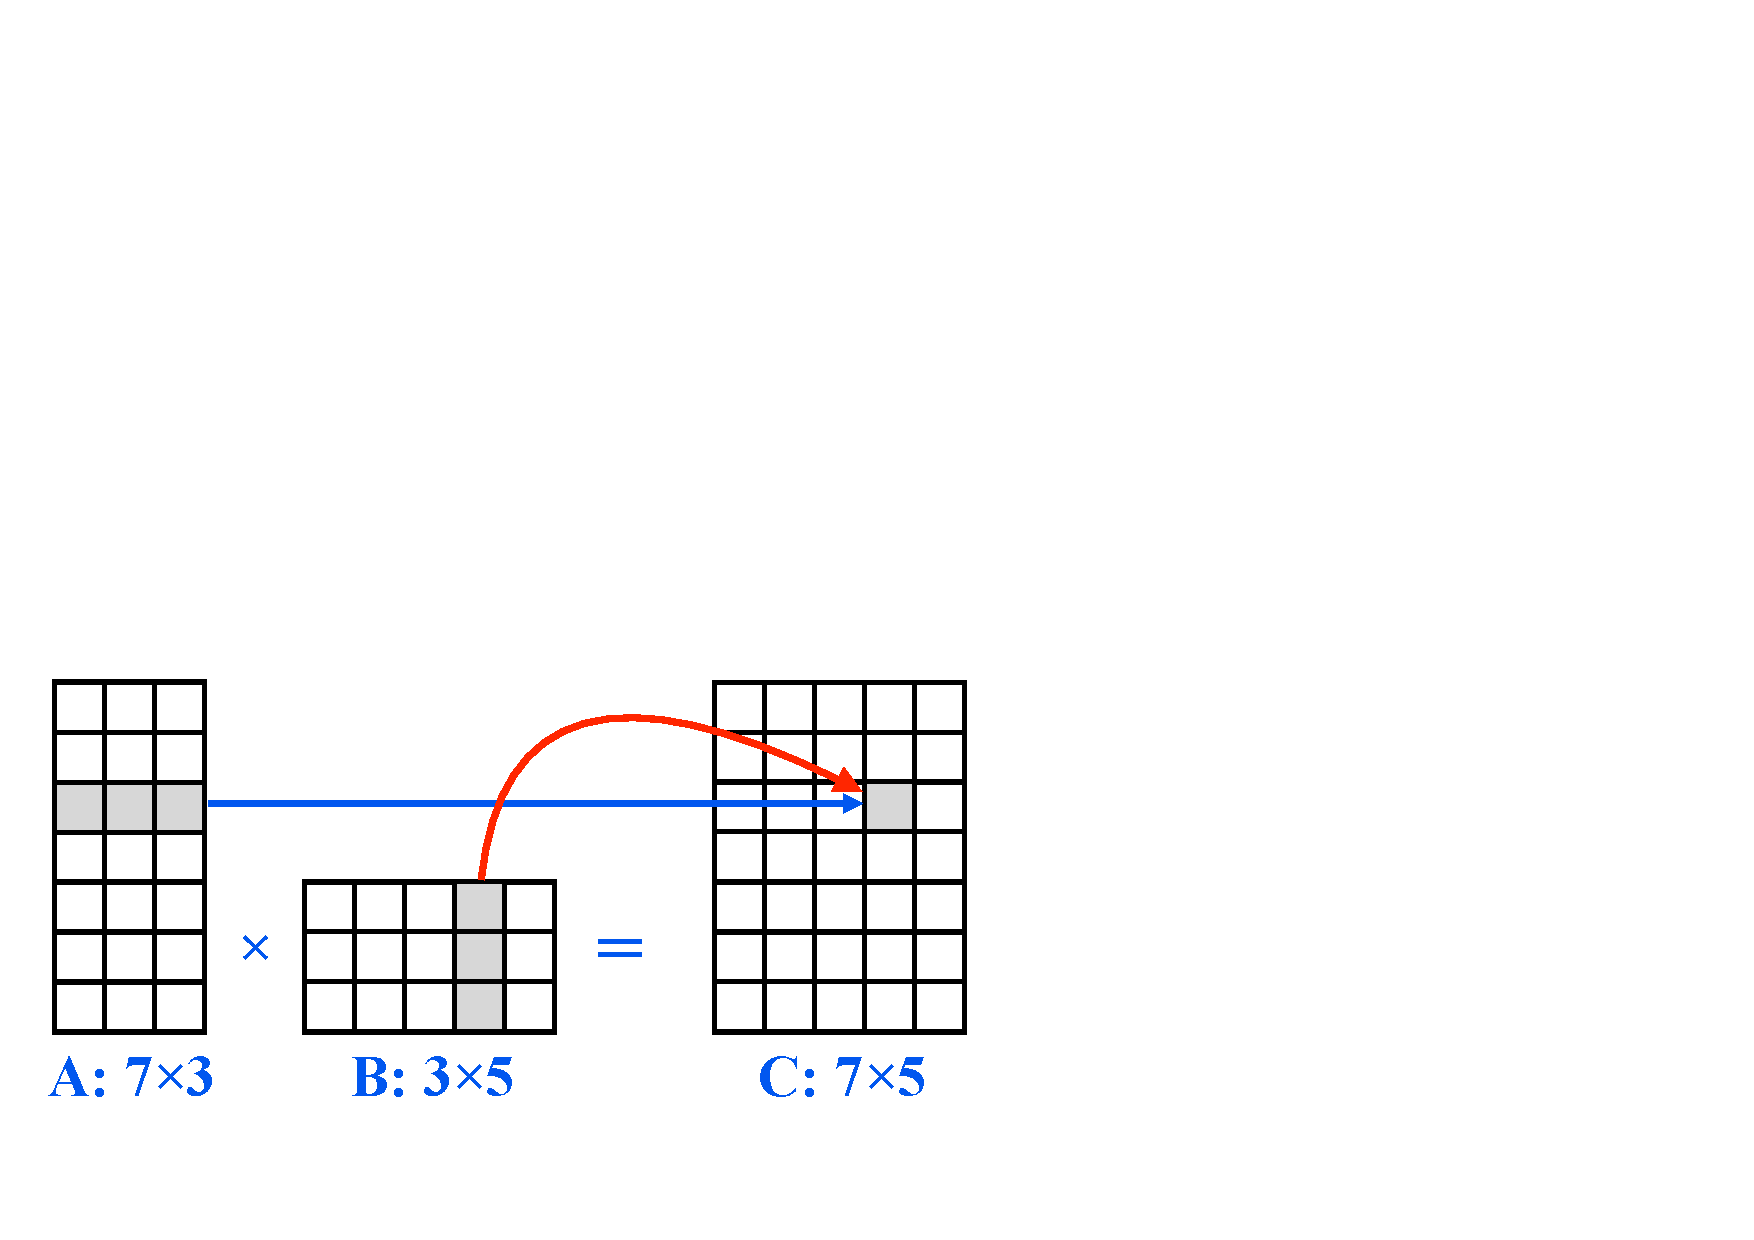
\includegraphics[width=0.60\textwidth]{matrix.pdf}
\end{center}

\end{frame}

%-------------------------------------------------------------------------
\begin{frame}{Approccio divide-et-impera}

\vspace{-9pt}
\small
\BB{Suddividiamo le matrici $n \times n$ in quattro matrici $n/2 \times n/2$}

\[
A = 
\begin{bmatrix} 
A_{1,1} & A_{1,2}\\	
A_{2,1} & A_{2,2} 
\end{bmatrix}
\qquad
B = 
\begin{bmatrix} 
B_{1,1} & B_{1,2}\\	
B_{2,1} & B_{2,2} 
\end{bmatrix}
\]

\medskip
\BB{Calcolo prodotto matrice}

\[
C = 
\begin{bmatrix} 
A_{1,1} \alert{\times} B_{1,1} + A_{1,2} \alert{\times} B_{2,1} & A_{1,1} \alert{\times} B_{1,2} + A_{1,2} \alert{\times} B_{2,2} \\
A_{2,1} \alert{\times} B_{1,1} + A_{2,2} \alert{\times} B_{2,1} & A_{2,1} \alert{\times} B_{1,2} + A_{2,2} \alert{\times} B_{2,2} \\
\end{bmatrix}
\]

\medskip
\BB{Equazione di ricorrenza}

\[
T(n) = \left\{ 
  \begin{array}{ll}
     1 & n = 1\\
     8T(n/2) + n^2  & n > 1 
  \end{array} 
\right.
\]

\end{frame}

%-------------------------------------------------------------------------
\begin{frame}{Algoritmo di Strassen}
\small
\vspace{-12pt}
\TwoCols{
\BB{Calcolo elementi intermedi}

\vspace{-12pt}
\begin{align*}
X_{1} &= (A_{11} + A_{22}) \alert{\times} (B_{11} + B_{22})\\
X_{2} &= (A_{21} + A_{22}) \alert{\times} B_{11}\\ 
X_{3} &= A_{11} \alert{\times} (B_{12} - B_{22})\\
X_{4} &= A_{22} \alert{\times} (B_{21} - B_{11})\\
X_{5} &= (A_{11} + A_{12}) \alert{\times} B_{22}\\
X_{6} &= (A_{21} - A_{11}) \alert{\times} (B_{11} + B_{12})\\
X_{7} &= (A_{12} - A_{22}) \alert{\times} (B_{21} + B_{22}).
\end{align*}
}
{
\BB{Equazione di ricorrenza}

\vspace{-12pt}
\begin{align*}
T(n) &= \left\{ 
  \begin{array}{ll}
     1 & n = 1\\
     7T(n/2) + n^2  & n > 1 
  \end{array} 
\right.\\
T(n) &= \Theta(n^{\log_2 7}) \approx \Theta(n^{2.81})
\end{align*}
}

\medskip
\BB{Calcolo matrice finale}

\[
C = 
\begin{bmatrix} 
 X_{1} + X_{4} - X_{5} + X_{7} & X_{3} + X_{5} \\
X_{2} + X_{4} & X_{1} + X_{3} - X_{2} + X_{6} \\
\end{bmatrix}
\]
\end{frame}

%-------------------------------------------------------------------------
\begin{frame}{Moltiplicazione matrici -- Panoramica storica}

\vspace{-9pt}
\begin{myboxtitle}[Algoritmo di Strassen (1969)]
\BI
\item $\Theta(n^{2.81})$
\item Il primo ad “scoprire” che era possibile moltiplicare due matrici in meno di $n^3$ 
moltiplicazioni scalari
\EI
\end{myboxtitle}

\begin{myboxtitle}[Coppersmith and Winograd (1990)]
\BI
\item $O(n^{2.37})$
\item Attuale algoritmo migliore
\item Fattori moltiplicativi molto alti
\EI
\end{myboxtitle}

\begin{myboxtitle}[Limite inferiore]
\BI
\item $\Omega(n^2)$
\EI
\end{myboxtitle}

\end{frame}

%-------------------------------------------------------------------------
\begin{frame}{Conclusioni}

\vspace{-9pt}
\BB{Quando applicare divide-et-impera}
\BIL
\item I passi “divide” e “combina” devono essere semplici
\item Ovviamente, i costi devono essere migliori del corrispondente algoritmo iterativo
\BI 
\item Esempio ok: sorting 
\item Esempio non ok: ricerca del minimo
\EI
\EIL

\medskip
\BB{Ulteriori vantaggi}
\BIL
\item Facile parallelizzazione
\item utilizzo ottimale della cache (“cache oblivious”)
\EIL

\end{frame}

\section{Esercizio}

\begin{frame}{Gap}

\vspace{-9pt}
\begin{myboxtitle}[Gap]
In un vettore $V$ contenente $n \geq 2$ interi, un \alert{gap} è un indice $i$, $1 < i \leq n$,
tale che $V[i-1]<V[i]$.
\begin{itemize}
\item Dimostrare che se $n \geq 2$ e $V[1]<V[n]$, allora $V$ contiene almeno un gap
\item Progettare un algoritmo che, dato un vettore $V$ contenente $n \geq 2$
interi e tale che $V[1]<V[n]$, restituisca la posizione di un gap nel vettore.
\end{itemize}
\end{myboxtitle}

\end{frame}

\begin{frame}{Gap}

Per assurdo:
\begin{itemize}
\item Supponiamo che non ci sia un gap nel vettore
\item Allora $V[1] \geq  V[2] \geq V[3] \geq \ldots \geq V[n-1] \geq V[n]$
\item Assurdo, perché $V[1]<V[n]$.
\end{itemize}
\end{frame}

\begin{frame}{Gap -- Dimostrazione per induzione}

Proviamo a riformulare la proprietà tenendo conto di due indici:
\BIL
\item Sia $V$ un vettore di dimensione $n$
\item Siano $i,j$ due indici tali che  
$1 \leq i < j \leq n$ e $V[i]<V[j]$
\EIL

\medskip
In altre parole, ci sono più di due elementi nel sottovettore
$V[i \ldots j]$ e il primo elemento $V[i]$ è più piccolo dell'ultimo
elemento $V[j]$.
\end{frame}

\begin{frame}{Gap -- Dimostrazione per induzione}

Vogliamo provare per induzione sulla dimensione $n$ del sottovettore che 
il sottovettore contiene un gap.
\BIL
\item \alert{Caso base}: $n=j-i+1=2$, i.e. $j = i+1$: \\
$V[i]<V[j]$ implica che $V[i] < V[i+1]$, che è un gap.
\item \alert{Ipotesi induttiva}: dato un qualunque (sotto)vettore $V[h \ldots k]$ di 
dimensione $n'<n$, tale che $V[h] < V[k]$, allora $V[h \ldots k]$ contiene un gap
\item \alert{Passo induttivo}: consideriamo un qualunque elemento
$m$ tale che $i<m<j$. Almeno uno dei due casi seguenti è vero:
\BI
\item Se $V[m] < V[j]$, allora esiste un gap in $V[m \ldots j]$, per ipotesi
induttiva
\item Se $V[i] < V[m]$, allora esiste un gap in $V[i \ldots m]$, per ipotesi
induttiva
\EI
\EIL

\end{frame}

\begin{frame}{Gap}

\vspace{-9pt}
\begin{Procedure}
\caption[A]{\INTEGER\ \textsf{gap}($\INTEGER[\,]\ V$, \INTEGER $n$)}
  \Return $\textsf{gapRec}(V, 1, n)$\;
\end{Procedure}

\begin{Procedure}
\caption[A]{\INTEGER\ \textsf{gapRec}($\INTEGER[\,]\ V$, \INTEGER $i$, \INTEGER $j$)}
\If{$j\Eq i+1$}{
	\Return $j$\;
}
\INTEGER\ $m = \lfloor (i+j)/2 \rfloor$\;
\eIf{$V[m] < V[j]$}{
	\Return $\textsf{gapRec}(V,m,j)$
}{
	\Return $\textsf{gapRec}(V,i,m)$
}

\end{Procedure}


\end{frame}

\begin{frame}{Performance evaluation}

\vspace{-9pt}
\begin{center}
\begin{tabular}{|r|r|r|}
\hline
$n$ & \textbf{Iterativa (ms)} & \textbf{Ricorsiva (${\mu}$s)}\\\hline
$10^3$ & 60.00 & 2.05\\\hline
$10^4$ & 610.00 & 2.78\\\hline
$10^5$ & 6\,110.00 & 3.36\\\hline
$10^6$ & 62\,440.00 & 4.01\\\hline
$10^7$ & 621\,690.00 & 4.87\\\hline
$10^8$ & 6\,205\,720.00 & 5.47\\\hline
\end{tabular}
\end{center}

\end{frame}




\end{document}



%-------------------------------------------------------------------------
\begin{frame}{}

\end{frame}
